\subsection{Grid search}\label{sec:appendix_grid_search}
We have run a grid search based on the standard model of the \gls{lda}, which allowed us to find an approximated optimal hyperparameter configuration.
We optimized for the best topic coherence measure during this grid search after 50 epochs, which was the number of epochs where the gains started to diminish.
\begin{figure}
	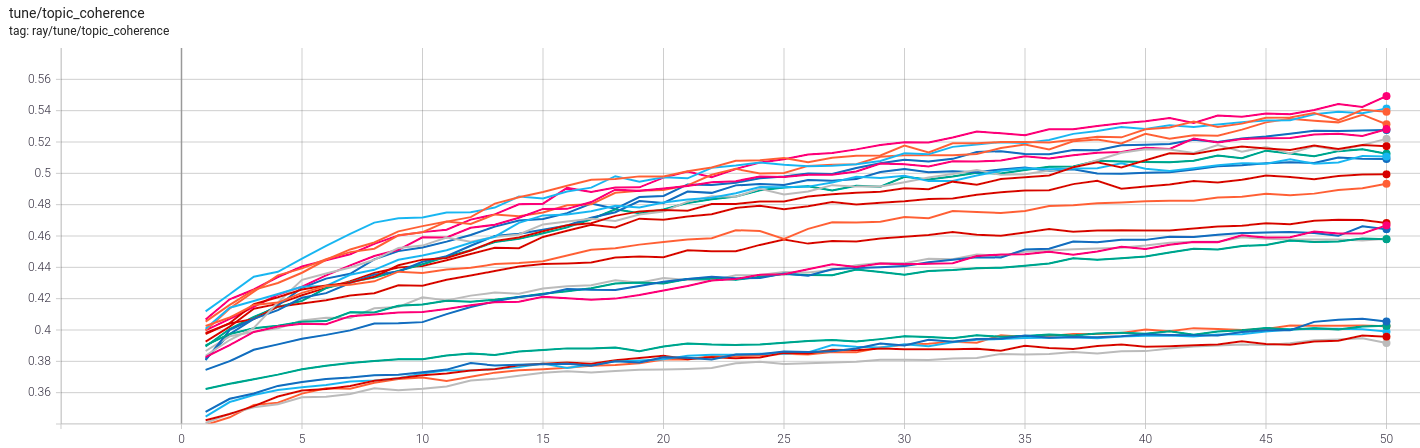
\includegraphics[width=\textwidth]{figures/gridsearch.png}
	\caption{Grid search over the $K_2$ parameters in \autoref{tab:gridsearch}.}
	\label{fig:visual_grid}
\end{figure} 
The five lowest values in \autoref{fig:visual_grid}, are where the $\alpha$ is $0.1$ and $\eta$ is $0.01$. 
This shows us that having the $\alpha$ high and the $\eta$ low does not yield good coherence results.
The next five values are where the $\alpha$ and $\eta$ are $0.01$, which also shows that a low value in both hyperparameters does not yield the best results either.
There is only a minor difference between the top configurations in \autoref{fig:visual_grid}, but the top two configurations are $70$ and $90$ topics.
The best hyperparameters are $K = 90$, $\alpha = 0.01$, and $\eta = 0.1$.
